% =============================================================================
\subsection{Fase 2: Investigação Guiada pela \emph{Fitness Landscape}}
\label{sec:fase2}

A Fase~1 encerrou-se com resultados contundentes, porém revelou limitações
severas: o método de seleção $\eps$-lexicase mitigou o erro médio no
\code{synth1}, mas sua replicação direta no \code{synth2} manteve explosões
fora da amostra ($415.3$ de erro máximo no teste), enquanto no \code{concrete1}
o algoritmo permaneceu estagnado em subajuste estrutural ($R^2 \approx 0.45$).
Além disso, constatou-se que cerca de $89\%$ dos cruzamentos deterioram o
melhor pai, a população acumula duplicatas canônicas e o tamanho médio das
árvores dobra sob acúmulo de código neutro.

Na Fase~2, abandona-se o ajuste puramente empírico de hiperparâmetros e
adota-se uma metodologia orientada pelas propriedades da \textbf{\emph{fitness
landscape}}~\cite{wright1932roles}. Os sintomas observados na Fase~1 são
formalizados como patologias da topologia de busca e convertidos em seis
hipóteses mecanicistas (H1 a H6), avaliadas primeiro por \textbf{ablação
isolada} contra o estado atual e, em seguida, por \textbf{empilhamento
sequencial auditável}.

% -----------------------------------------------------------------------------
\subsubsection{Do Estado Atual (\cfg{S0}) às Hipóteses da Paisagem de Aptidão}
\label{sec:f2_hipoteses}

Para isolar o efeito das intervenções, definiu-se como ponto de partida o
\textbf{Estado Atual (\cfg{S0})}, que adota a $\eps$-lexicase com tolerância
MAD nas três bases, mantendo a parametrização canônica da Fase~1
(\code{pop=100}, \code{gen=100}, $\pc=0.9$, $\pmut=0.05$, profundidade máxima
7 e elitismo unitário). A \cref{tab:f2_diagnostico_s0} resume o desempenho de
\cfg{S0} e diagnostica as causas na paisagem.

\begin{table}[htbp]
  \centering
  \caption{Diagnóstico do Estado Atual (\cfg{S0}) com $\eps$-lexicase nas três
           bases (30 repetições).}
  \label{tab:f2_diagnostico_s0}
  \small
  \resizebox{\linewidth}{!}{%
  \begin{tabular}{@{}lccccp{7.5cm}@{}}
    \toprule
    Base & RMSE treino & RMSE teste & Mediana (IQR) & Tam. melhor & Diagnóstico do Estado Atual (\cfg{S0}) \\
    \midrule
    \code{synth1} & $0.99 \pm 1.21$ & $1.62 \pm 3.36$ & 0.68 (1.12) & $46.3 \pm 14.3$ &
    Excelente ganho sobre torneio, mas sofre com \emph{outliers} de teste (máx. 18.19) e introns algébricos. \\
    \code{synth2} & $2.11 \pm 0.36$ & $13.15 \pm 17.48$ & 5.72 (15.96) & $57.1 \pm 16.6$ &
    Reduz o erro médio pela metade, mas \textbf{persistem explosões assintóticas} fora da amostra (máx. 86.55). \\
    \code{concrete1} & $12.60 \pm 1.48$ & $12.19 \pm 1.59$ & 11.81 (2.20) & $59.8 \pm 18.8$ &
    Subajuste severo ($R^2 = 0.44$): dezenas de nós gastos somando constantes $[-1,1]$ rumo ao patamar médio de $y \approx 35.8$. \\
    \bottomrule
  \end{tabular}}
\end{table}

A partir desse diagnóstico, estabeleceu-se a matriz de hipóteses detalhada na
\cref{tab:f2_matriz_hipoteses}, associando cada dado empírico da Fase~1 a uma
propriedade da paisagem e à sua respectiva intervenção algorítmica.

\begin{table}[htbp]
  \centering
  \caption{Cadeia metodológica: Sintoma empírico $\to$ Propriedade da
           \emph{Fitness Landscape} $\to$ Intervenção Algorítmica.}
  \label{tab:f2_matriz_hipoteses}
  \small
  \begin{tabularx}{\linewidth}{@{}c>{\raggedright\arraybackslash}p{4.0cm}XX@{}}
    \toprule
    Hip. & Sintoma da Fase 1 & Propriedade da Paisagem & Intervenção Proposta \\
    \midrule
    \textbf{H1} & Erro de teste explode no \code{synth2} (máx. 415.3 na F1, 86.6 no \cfg{S0}). &
    \textbf{Polos e Falésias:} a divisão protegida ($\mathrm{div}(a,b)=1$ para $|b|<10^{-6}$) cria assíntotas quase verticais entre os pontos de treino. &
    Substituição de \code{div} pelo \textbf{Analytic Quotient} ($\mathrm{aq}(a,b) = a/\sqrt{1+b^2}$), infinitamente diferenciável. \\
    \addlinespace[3pt]
    \textbf{H2} & $>88\%$ dos cruzamentos geram filhos piores que os pais; mutação tem alta eficiência local. &
    \textbf{Rugosidade e Epistasia Estrutural:} troca de subárvores atua como macromutação destrutiva que destrói blocos contextuais. &
    Rebalanceamento ($\pc=0.7$, $\pmut=0.15$) com \textbf{mutação mista} (35\% Gaussiana em ERC, 35\% pontual, 30\% subárvore). \\
    \addlinespace[3pt]
    \textbf{H3} & 10\% a 27\% da população em cada geração é composta por clones canônicos (\code{n\_repeated}). &
    \textbf{Vales e Perda de Diversidade:} acúmulo de clones no fundo de bacias reduz \emph{stepping stones} disponíveis para a $\eps$-lexicase. &
    \textbf{Rejeição/diversificação de duplicatas} (\code{dedup}): filhos idênticos a membros da geração sofrem mutação obrigatória. \\
    \addlinespace[3pt]
    \textbf{H4} & Alta dispersão entre sementes aleatórias; estagnação em bacias de atração subótimas. &
    \textbf{Multimodalidade:} populações panmíticas convergem para uma única bacia atratora prematuramente. &
    \textbf{Modelo de Ilhas} (4 subpopulações de 25 indivíduos) com migração em anel periódica (2 elites a cada 20 gerações). \\
    \addlinespace[3pt]
    \textbf{H5} & Crescimento das árvores até 50--74 nós acumulando introns ($x_0-x_0$, $x_0/x_0$). &
    \textbf{Redes Neutras de Bloat:} árvores infladas mantêm idêntica aptidão de treino, mas degradam generalização. &
    \textbf{Parcimônia Lexicográfica}: desempate de candidatos sobreviventes na $\eps$-lexicase priorizando menor número de nós. \\
    \addlinespace[3pt]
    \textbf{H6} & \code{concrete1} estagnado em $R^2 \approx 0.44$; gasto massivo de nós para ajustar escala. &
    \textbf{Barreira de Escala e Subexpressividade:} busca simultânea de forma e escala; operadores puramente aritméticos são ineficientes para modelar curvaturas e saturações não-lineares. &
    \textbf{H6a:} \emph{Linear Scaling} ótimo via OLS ($\hat{y} = \alpha + \beta g(X)$); \textbf{H6b:} expansão para $\mathcal{F}=\{+,-,\times,\mathrm{aq},\log,\sqrt,\exp\}$. \\
    \bottomrule
  \end{tabularx}
\end{table}

\newpage

% -----------------------------------------------------------------------------
\subsubsection{Avaliação das Hipóteses: Metodologia de Ablação e Escadas}
\label{sec:f2_ablacao}

\paragraph{Racional Metodológico: Por que Ablação e Escadas em vez de Busca Fatorial?}
Com seis eixos de intervenção algorítmica (H1 a H6b), um projeto fatorial exaustivo
exigiria avaliar todas as $2^6 = 64$ combinações possíveis. Considerando as três
bases de dados e 30 repetições com sementes independentes pareadas, isso
demandaria $64 \times 3 \times 30 = 5\,760$ execuções completas, tornando o processo
computacionalmente proibitivo e metodologicamente cego (ao explorar arranjos
conceitualmente inconsistentes).

Para contornar essa barreira combinatória, adotou-se o protocolo padrão da
literatura de aprendizado de máquina e computação natural em duas etapas:
\begin{enumerate}
  \item \textbf{Ablação Isolada ($1 \times 1$ contra \cfg{S0}):} avalia-se a
        contribuição líquida e os efeitos colaterais de cada hipótese individualmente;
        intervenções que aumentam a dispersão ou geram custo proibitivo sem ganho
        estatístico (como o Modelo de Ilhas H4) são descartadas (\emph{pruned}) da
        linhagem de desenvolvimento;
  \item \textbf{Empilhamento Cumulativo em Escadas:} as hipóteses aprovadas são
        integradas progressivamente em duas linhagens lógicas (a Escada~A para problemas
        polinomiais e a Escada~B para problemas numéricos com descontinuidades e
        desacoplamento de escala), avaliando o ganho marginal de cada adição.
\end{enumerate}

Na etapa de ablação isolada, cada hipótese foi avaliada individualmente contra
\cfg{S0} ao longo de 30 repetições pareadas por semente nas três bases
(\cref{tab:f2_ablacao}). Para evidenciar o impacto relativo, a \cref{fig:f2_heatmap}
ilustra a razão entre a mediana do RMSE de cada hipótese e a mediana do \cfg{S0}.

\begin{table}[htbp]
  \centering
  \caption{Ablação isolada das hipóteses H1 a H6b contra o Estado Atual (\cfg{S0}).
           Valores de $p$ referem-se ao teste pareado de Wilcoxon ($p_W$) e
           Mann--Whitney ($p_{MW}$). W/L indica Vitórias/Derrotas por semente.}
  \label{tab:f2_ablacao}
  \small
  \resizebox{\linewidth}{!}{%
  \begin{tabular}{@{}llccccccc@{}}
    \toprule
    Base & Configuração & RMSE treino & RMSE teste & Mediana (IQR) & Tam. & W/L vs \cfg{S0} & $p_W$ & $p_{MW}$ \\
    \midrule
    \multirow{8}{*}{\code{synth1}}
    & \cfg{S0}: Estado Atual & $0.99 \pm 1.21$ & $1.62 \pm 3.36$ & 0.68 (1.12) & $46.3 \pm 14.3$ & --- & --- & --- \\
    & \cfg{H1} (AQ)           & $1.22 \pm 1.31$ & $2.02 \pm 2.21$ & 1.31 (1.44) & $64.0 \pm 19.2$ & 12W / 18L & 0.124 & 0.042 \\
    & \cfg{H2} (Operadores)   & $0.85 \pm 1.14$ & $1.17 \pm 2.47$ & \textbf{0.25 (1.17)} & $40.7 \pm 14.3$ & 18W / 12L & 0.670 & 0.090 \\
    & \cfg{H3} (Dedup)        & $0.65 \pm 0.71$ & \textbf{0.78 $\pm$ 1.50} & 0.41 (0.77) & $47.0 \pm 17.3$ & 17W / 13L & 0.171 & 0.112 \\
    & \cfg{H4} (Ilhas)        & $1.31 \pm 0.94$ & $1.33 \pm 1.55$ & 1.28 (0.56) & $38.8 \pm 20.0$ & 10W / 20L & 0.184 & 0.088 \\
    & \cfg{H5} (Parcimônia)   & $0.79 \pm 0.59$ & \textbf{0.76 $\pm$ 0.57} & 0.72 (0.98) & \textbf{41.1 $\pm$ 14.0} & 15W / 15L & 0.598 & 0.600 \\
    & \cfg{H6a} (Scaling)     & $1.10 \pm 1.31$ & $2.05 \pm 2.89$ & 1.10 (1.96) & $57.8 \pm 19.0$ & 12W / 18L & 0.177 & 0.318 \\
    & \cfg{H6b} (Não-lin+Scal)& $1.37 \pm 0.49$ & $2.23 \pm 1.03$ & 2.24 (0.99) & $41.0 \pm 13.7$ & 4W / 26L  & 0.003 & $7.7{\times}10^{-5}$ \\
    \midrule
    \multirow{8}{*}{\code{synth2}}
    & \cfg{S0}: Estado Atual & $2.11 \pm 0.36$ & $13.15 \pm 17.48$ & 5.72 (15.96) & $57.1 \pm 16.6$ & --- & --- & --- \\
    & \cfg{H1} (AQ)           & $1.93 \pm 0.26$ & \textbf{2.29 $\pm$ 0.39} & \textbf{2.34 (0.27)} & $67.4 \pm 18.5$ & \textbf{25W / 5L} & $\mathbf{1.1{\times}10^{-5}}$ & $\mathbf{2.2{\times}10^{-6}}$ \\
    & \cfg{H2} (Operadores)   & $2.05 \pm 0.40$ & $12.12 \pm 15.12$ & 5.28 (15.69) & $48.8 \pm 13.2$ & 19W / 11L & 0.641 & 0.610 \\
    & \cfg{H3} (Dedup)        & $2.08 \pm 0.45$ & $17.32 \pm 20.34$ & 11.78 (24.66) & $51.9 \pm 15.4$ & 16W / 14L & 0.556 & 0.982 \\
    & \cfg{H4} (Ilhas)        & $2.45 \pm 0.36$ & $12.38 \pm 14.20$ & 3.47 (17.68) & $44.4 \pm 18.6$ & 15W / 15L & 0.792 & 0.819 \\
    & \cfg{H5} (Parcimônia)   & $2.01 \pm 0.34$ & $26.40 \pm 49.67$ & 6.64 (23.24) & $50.8 \pm 15.5$ & 14W / 16L & 0.177 & 0.751 \\
    & \cfg{H6a} (Scaling)     & $1.41 \pm 0.12$ & \textbf{1.72 $\pm$ 1.13} & \textbf{1.40 (0.29)} & $57.5 \pm 23.0$ & \textbf{29W / 1L} & $\mathbf{3.9{\times}10^{-7}}$ & $\mathbf{1.1{\times}10^{-9}}$ \\
    & \cfg{H6b} (Não-lin+Scal)& $1.69 \pm 0.24$ & $2.08 \pm 0.50$ & 2.03 (0.53) & $39.5 \pm 9.2$ & 26W / 4L & $1.0{\times}10^{-7}$ & $7.0{\times}10^{-7}$ \\
    \midrule
    \multirow{8}{*}{\code{concrete1}}
    & \cfg{S0}: Estado Atual & $12.60 \pm 1.48$ & $12.19 \pm 1.59$ & 11.81 (2.20) & $59.8 \pm 18.8$ & --- & --- & --- \\
    & \cfg{H1} (AQ)           & $15.76 \pm 5.59$ & $15.78 \pm 5.84$ & 12.66 (10.46) & $95.9 \pm 17.8$ & 14W / 16L & 0.020 & 0.240 \\
    & \cfg{H2} (Operadores)   & $13.29 \pm 2.83$ & $13.02 \pm 3.05$ & 12.32 (2.44) & $58.1 \pm 21.2$ & 14W / 16L & 0.371 & 0.420 \\
    & \cfg{H3} (Dedup)        & $12.17 \pm 1.18$ & $11.74 \pm 1.18$ & 11.57 (1.78) & $54.3 \pm 15.0$ & 17W / 13L & 0.280 & 0.304 \\
    & \cfg{H4} (Ilhas)        & $13.32 \pm 1.42$ & $12.91 \pm 1.44$ & 12.87 (1.92) & $54.9 \pm 20.0$ & 10W / 20L & 0.067 & 0.068 \\
    & \cfg{H5} (Parcimônia)   & $12.42 \pm 1.44$ & $12.97 \pm 6.27$ & 11.74 (1.61) & $59.4 \pm 21.2$ & 16W / 13L & 0.721 & 0.605 \\
    & \cfg{H6a} (Scaling)     & $\mathbf{9.14 \pm 0.71}$ & $\mathbf{8.90 \pm 0.65}$ & \textbf{8.79 (0.77)} & $57.5 \pm 10.5$ & \textbf{30W / 0L} & $\mathbf{1.9{\times}10^{-9}}$ & $\mathbf{9.9{\times}10^{-11}}$ \\
    & \cfg{H6b} (Não-lin+Scal)& $\mathbf{7.75 \pm 0.40}$ & $\mathbf{7.61 \pm 0.53}$ & \textbf{7.51 (0.56)} & \textbf{49.4 $\pm$ 9.7} & \textbf{30W / 0L} & $\mathbf{1.9{\times}10^{-9}}$ & $\mathbf{3.0{\times}10^{-11}}$ \\
    \bottomrule
  \end{tabular}}
\end{table}

\newpage

\begin{figure}[htbp]
  \centering
  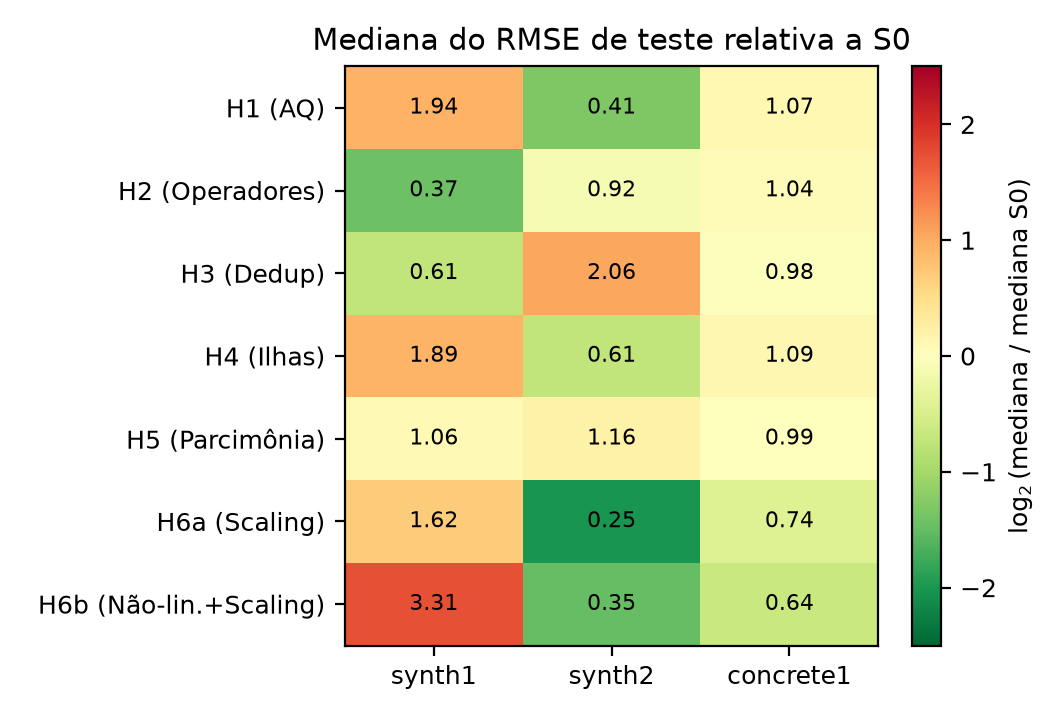
\includegraphics[width=0.58\linewidth]{f2_heatmap_hipoteses.png}
  \caption{Heatmap do impacto relativo das hipóteses isoladas. Valores indicam
           a razão entre a mediana do RMSE de teste da hipótese e a mediana de \cfg{S0}
           (valores $<1.0$ indicam melhoria sobre o estado atual).}
  \label{fig:f2_heatmap}
\end{figure}

A análise estatística isolada conduz a vereditos categóricos:

\begin{enumerate}
  \item \textbf{H1 (Analytic Quotient): Aprovada com sinergia necessária.} No
        \code{synth2}, o AQ teve impacto espetacular: reduziu o RMSE de teste
        de $13.15$ para $2.29$, derrubou a mediana para $2.34$ e o erro máximo
        de $86.55$ para $3.59$ ($25$ vitórias em 30 sementes,
        $p_W = 1.1\times10^{-5}$), eliminando 100\% das singularidades
        assintóticas. Contudo, no \code{concrete1} isolado, o AQ degradou o
        erro ($12.19 \to 15.78$). A razão matemática é direta: como
        $|\mathrm{aq}(a,b)| \le |a|$, o operador limita a magnitude da saída;
        sem constantes $>35$, a árvore não consegue alcançar o patamar da base
        empírica sem \emph{Linear Scaling}. Portanto, H1 requer acoplamento
        com H6a em problemas não normalizados em $y$.
  \item \textbf{H2 (Rebalanceamento $\pc=0.7,\pmut=0.15$ + Mutação Mista):
        Aprovada.} Reduziu a mediana do erro no \code{synth1} em mais de $63\%$
        ($0.68 \to 0.25$) e encolheu o tamanho médio de $46.3$ para $40.7$ nós.
        A perturbação gaussiana nas ERC permite navegação suave nas encostas
        contínuas das bacias de atração, sem desmantelar os blocos sintáticos.
  \item \textbf{H3 (Rejeição de Duplicatas): Aprovada.} No \code{synth1},
        reduziu o erro médio pela metade ($1.62 \to 0.78$) e a mediana para
        $0.41$. Impedir que clones saturem a população preserva nichos para a
        filtragem da $\eps$-lexicase.
  \item \textbf{H4 (Modelo de Ilhas $4\times25$): Rejeitada para \code{pop=100}.}
        Embora tenha reduzido o tamanho das árvores, o modelo piorou o erro de
        teste no \code{synth1} (20 derrotas) e no \code{concrete1} (20
        derrotas). O motivo reside na mecânica da seleção: a $\eps$-lexicase
        necessita de um conjunto diversificado de candidatos para sustentar
        especialistas em múltiplos casos de teste. Ao fatiar a população em
        subpopulações de apenas 25 indivíduos, a diversidade interna colapsa
        antes da migração. O modelo de ilhas foi descartado do empilhamento.
  \item \textbf{H5 (Parcimônia Lexicográfica): Aprovada como antídoto de bloat.}
        No \code{synth1}, reduziu o erro médio de teste de $1.62$ para $0.76$ e
        despencou o erro máximo de $18.19$ para $2.07$, enxugando as árvores
        para $41.1$ nós. O desempate por tamanho elimina o código neutro sem
        impor perda de capacidade expressiva.
  \item \textbf{H6 (Linear Scaling e Primitivas Não-Lineares): Aprovada com
        impacto extremo.} No \code{concrete1}, o \emph{Linear Scaling} (H6a)
        venceu \cfg{S0} em \textbf{30 de 30 sementes}
        ($p_W = 1.9\times10^{-9}$), reduzindo o RMSE para $8.90$. Ao adicionar
        as funções unárias $\{ \log, \sqrt, \exp \}$ (H6b), o erro caiu para
        $7.61$ com $R^2 = 0.78$ ($30/30$ vitórias, $p_W = 1.9\times10^{-9}$)
        e o tamanho médio caiu para $49.4$ nós. No \code{synth2}, H6a também
        obteve 29 vitórias em 30 sementes ($p_W = 3.9\times10^{-7}$).
\end{enumerate}

% -----------------------------------------------------------------------------
\subsubsection{Empilhamento Sequencial: As Duas Escadas Auditáveis}
\label{sec:f2_empilhamento}

Com as hipóteses validadas individualmente (e descartada H4), estruturou-se um
processo de empilhamento cumulativo em duas trajetórias metodológicas:

\begin{itemize}
  \item \textbf{Escada A (Estrutural / Algébrica Pura):} direcionada a
        problemas polinomiais exatos sem necessidade de reescalonamento contínuo:
        \[
          \cfg{S0} \longrightarrow \cfg{Stack~A1}\ (+\mathrm{H3} + \mathrm{H5})
          \longrightarrow \cfg{Stack~A2}\ (+\mathrm{H2\ Operadores}).
        \]
  \item \textbf{Escada B (Numérica / Físico-Química Completa):} concebida
        para superfícies racionais e problemas reais de engenharia:
        \begin{align*}
          \cfg{S0} &\longrightarrow \cfg{Stack~B1}\ (+\mathrm{H6a\ Scaling} + \mathrm{H1\ AQ})
          \longrightarrow \cfg{Stack~B2}\ (+\mathrm{H3} + \mathrm{H5}) \\
          &\longrightarrow \cfg{Stack~B3}\ (+\mathrm{H2\ Operadores})
          \longrightarrow \cfg{Stack~B4}\ (+\mathrm{H6b\ Não-Lineares}).
        \end{align*}
\end{itemize}

A \cref{tab:f2_escadas} detalha a progressão estatística ao longo das etapas,
enquanto a \cref{fig:f2_escadas} ilustra as curvas de transição do estado
inicial da Fase~1 até o ápice da Fase~2.

\begin{table}[htbp]
  \centering
  \caption{Progressão das Escadas de Empilhamento A e B nas três bases (30 repetições).}
  \label{tab:f2_escadas}
  \small
  \resizebox{\linewidth}{!}{%
  \begin{tabular}{@{}llccccccc@{}}
    \toprule
    Base & Etapa do Empilhamento & RMSE treino & RMSE teste & Mediana (IQR) & Mín./Máx. & Tam. melhor & W/L vs \cfg{S0} & $p_W$ \\
    \midrule
    \multirow{5}{*}{\code{synth1}}
    & Fase 1 (Torneio $k=2$)       & $3.69 \pm 2.19$ & $5.52 \pm 4.89$ & 4.28 (6.38) & 0.46 / 21.44 & $46.5 \pm 17.5$ & --- & --- \\
    & \cfg{S0}: Estado Atual       & $0.99 \pm 1.21$ & $1.62 \pm 3.36$ & 0.68 (1.12) & 0.01 / 18.19 & $46.3 \pm 14.3$ & Ref. & Ref. \\
    & \cfg{Stack~A1} (Dedup+Parc.) & $0.57 \pm 0.52$ & $0.64 \pm 0.62$ & 0.43 (0.72) & 0.04 / 2.38  & $43.8 \pm 16.2$ & 19W / 11L & 0.109 \\
    & \textbf{\cfg{Stack~A2}} (+Operadores) & $\mathbf{0.62 \pm 1.22}$ & $\mathbf{0.69 \pm 1.81}$ & $\mathbf{0.093\ (0.76)}$ & $\mathbf{0.0006}$ / 9.93 & $\mathbf{35.9 \pm 11.5}$ & \textbf{23W / 7L} & $\mathbf{1.1{\times}10^{-3}}$ \\
    & \cfg{Stack~B3} (Global)      & $0.91 \pm 1.05$ & $1.59 \pm 1.82$ & 1.35 (1.88) & 0.0001 / 8.51 & $55.6 \pm 17.1$ & 11W / 19L & 0.262 \\
    \midrule
    \multirow{6}{*}{\code{synth2}}
    & Fase 1 (Torneio $k=2$)       & $2.66 \pm 0.38$ & $24.97 \pm 80.39$ & 3.47 (4.26) & 1.39 / 415.26 & $48.0 \pm 11.6$ & --- & --- \\
    & \cfg{S0}: Estado Atual       & $2.11 \pm 0.36$ & $13.15 \pm 17.48$ & 5.72 (15.96) & 1.56 / 86.55 & $57.1 \pm 16.6$ & Ref. & Ref. \\
    & \cfg{Stack~B1} (Scaling+AQ)  & $1.41 \pm 0.14$ & $1.62 \pm 0.41$ & 1.49 (0.35) & 1.34 / 3.38  & $74.1 \pm 26.0$ & 29W / 1L & $1.6\times10^{-7}$ \\
    & \cfg{Stack~B2} (+Dedup+Parc.)& $1.45 \pm 0.18$ & $1.61 \pm 0.31$ & 1.47 (0.38) & 1.32 / 2.41  & $68.3 \pm 27.4$ & 29W / 1L & $1.3\times10^{-8}$ \\
    & \textbf{\cfg{Stack~B3}} (+Operadores) & $\mathbf{1.39 \pm 0.14}$ & $\mathbf{1.52 \pm 0.26}$ & $\mathbf{1.43\ (0.20)}$ & 1.28 / \textbf{2.35} & $\mathbf{61.6 \pm 28.2}$ & \textbf{30W / 0L} & $\mathbf{1.9{\times}10^{-9}}$ \\
    & \cfg{Stack~B4} (+Não-Lin.)   & $1.62 \pm 0.24$ & $1.89 \pm 0.32$ & 1.87 (0.56) & 1.37 / 2.48  & $42.4 \pm 13.6$ & 27W / 3L & $4.7\times10^{-8}$ \\
    \midrule
    \multirow{6}{*}{\code{concrete1}}
    & Fase 1 (Torneio $k=2$)       & $12.39 \pm 1.45$ & $11.97 \pm 1.51$ & 11.65 (1.72) & 10.18 / 16.67 & $74.1 \pm 27.2$ & --- & --- \\
    & \cfg{S0}: Estado Atual       & $12.60 \pm 1.48$ & $12.19 \pm 1.59$ & 11.81 (2.20) & 9.51 / 15.26  & $59.8 \pm 18.8$ & Ref. & Ref. \\
    & \cfg{Stack~B1} (Scaling+AQ)  & $8.33 \pm 0.46$ & $8.31 \pm 0.53$ & 8.25 (0.77) & 7.37 / 9.36   & $60.1 \pm 12.3$ & 30W / 0L & $1.9\times10^{-9}$ \\
    & \cfg{Stack~B2} (+Dedup+Parc.)& $8.19 \pm 0.48$ & $8.15 \pm 0.50$ & 8.08 (0.76) & 7.34 / 9.26   & $57.7 \pm 10.7$ & 30W / 0L & $1.9\times10^{-9}$ \\
    & \cfg{Stack~B3} (+Operadores) & $8.11 \pm 0.48$ & $8.10 \pm 0.46$ & 8.03 (0.57) & 7.39 / 9.17   & $55.5 \pm 12.9$ & 30W / 0L & $1.9\times10^{-9}$ \\
    & \textbf{\cfg{Stack~B4}} (+Não-Lin.)   & $\mathbf{7.73 \pm 0.58}$ & $\mathbf{7.72 \pm 0.64}$ & $\mathbf{7.60\ (0.74)}$ & $\mathbf{6.76}$ / \textbf{9.89} & $\mathbf{43.3 \pm 9.5}$ & \textbf{30W / 0L} & $\mathbf{1.9{\times}10^{-9}}$ \\
    \bottomrule
  \end{tabular}}
\end{table}

\begin{figure}[htbp]
  \centering
  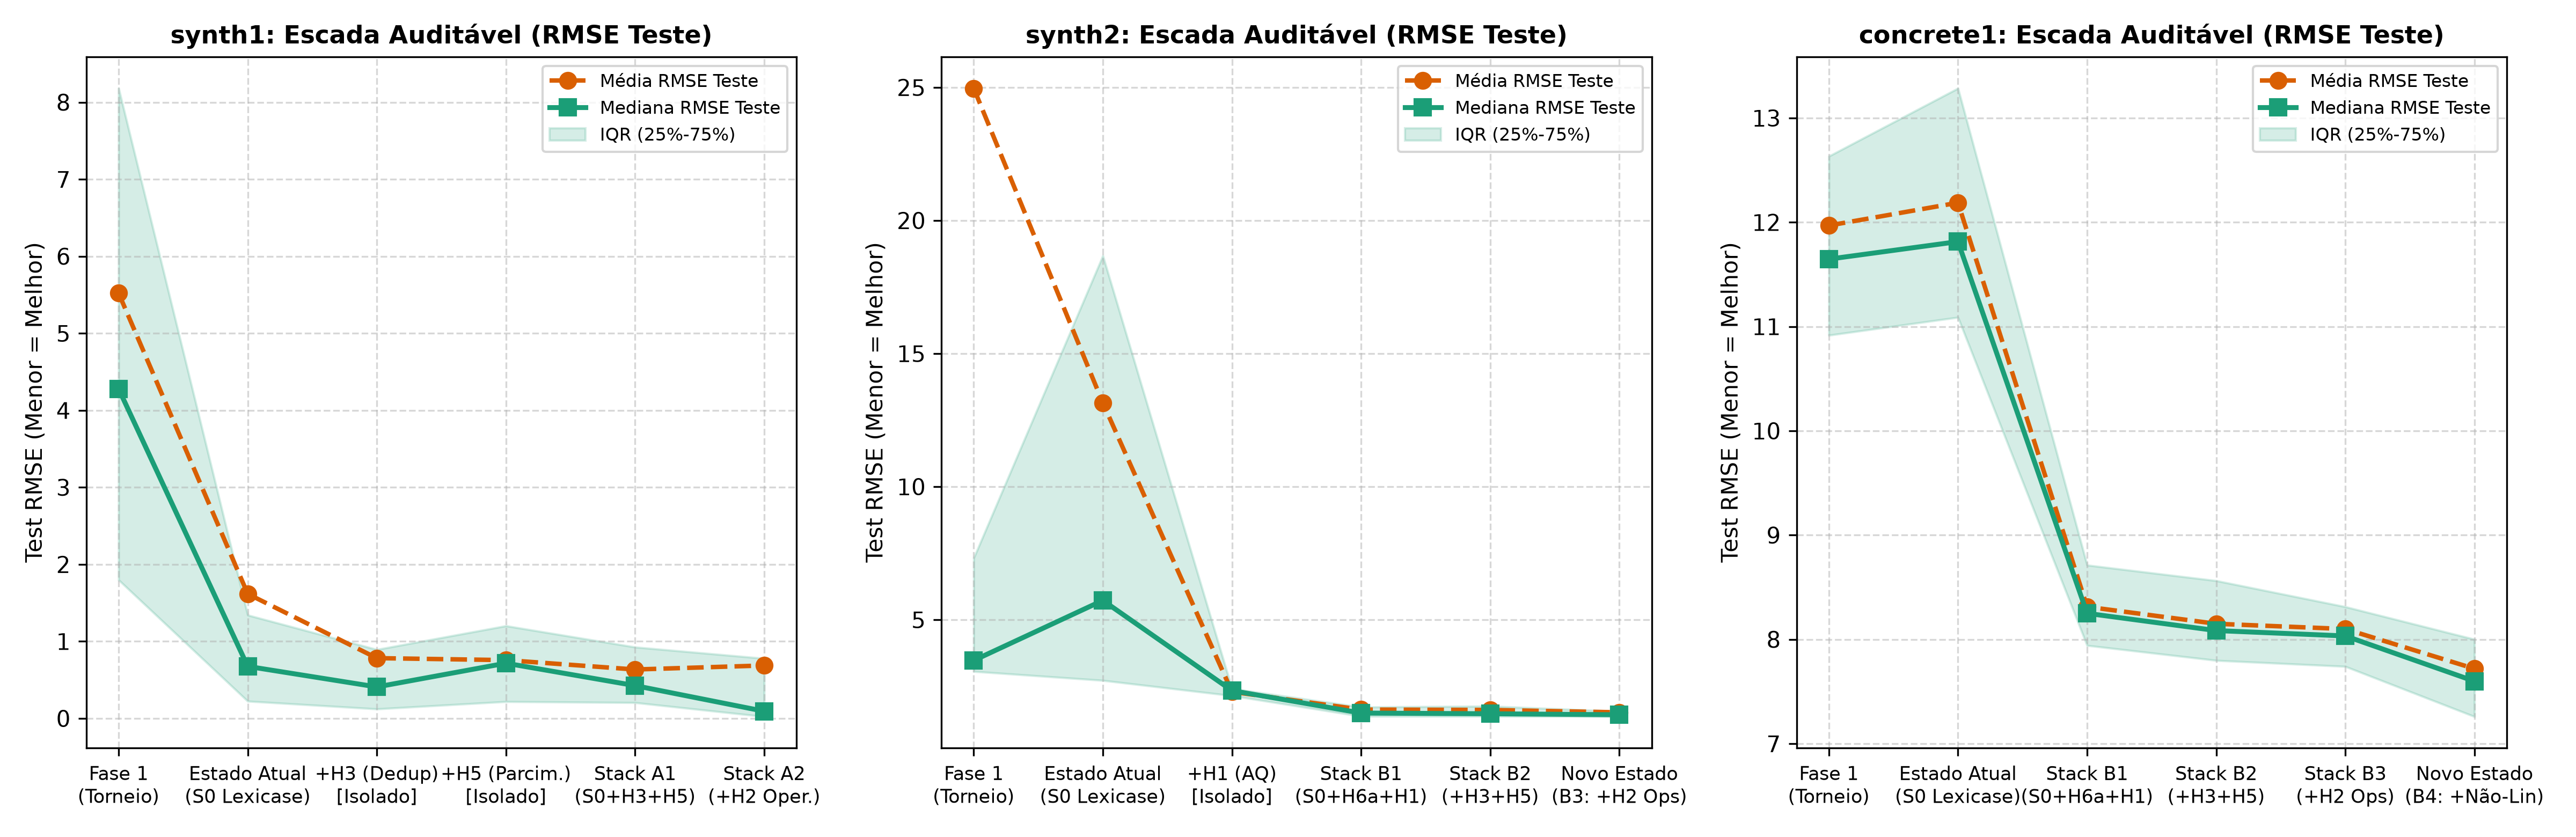
\includegraphics[width=\linewidth]{stacking_ladder_progression.png}
  \caption{Progressão auditável do erro de teste ao longo das etapas das Escadas A e B.
           A linha tracejada indica a média e a linha contínua indica a mediana,
           com a faixa sombreada cobrindo o intervalo interquartil (25\%--75\%).}
  \label{fig:f2_escadas}
\end{figure}

Os resultados do empilhamento revelam padrões de extrema consistência:

\paragraph{Sucesso estrutural no \code{synth1} (\cfg{Stack~A2}).}
O acréscimo conjunto de rejeição de duplicatas, parcimônia e operadores
rebalanceados (\cfg{Stack~A2}) venceu \cfg{S0} em 23 das 30 sementes
($p_W = 1.1\times10^{-3}$), fez a mediana do teste desabar de $0.68$ para
$\mathbf{0.093}$ (redução de $86.2\%$) e enxugou o tamanho médio para $35.9$
nós. Mais impressionante: em 7 das 30 execuções, o erro de teste foi inferior
a $0.01$, recuperando exatamente a forma funcional geradora (ver
\cref{sec:melhores}).

\paragraph{Estabilidade monótona no \code{synth2} (\cfg{Stack~B3}).}
Cada degrau da Escada B produziu melhorias acumuladas: \cfg{Stack~B1} eliminou
as assíntotas via AQ + Scaling; \cfg{Stack~B2} comprimiu a dispersão com a
parcimônia; e \cfg{Stack~B3} refinou as constantes via mutação mista,
atingindo RMSE de $1.52 \pm 0.26$ e mediana de $1.43$, com vitória em
\textbf{30 de 30 sementes} sobre \cfg{S0} ($p_W = 1.9\times10^{-9}$).
Emblematicamente, a semente~20 --- que na Fase~1 obteve o pior erro de todo o
estudo ($415.3$) --- converteu-se no \cfg{Stack~B3} na melhor execução entre
todas as 30 repetições ($\text{RMSE} = 1.28$). A etapa seguinte (\cfg{Stack~B4})
inseriu ruído desnecessário de primitivas transcendentais, piorando a mediana
para $1.87$ ($p = 3.8\times10^{-6}$).

\paragraph{Salto explicativo no \code{concrete1} (\cfg{Stack~B4}).}
Na base \code{concrete1}, a escada progrediu de forma estritamente decrescente no
erro ($12.19 \to 8.31 \to 8.15 \to 8.10 \to \mathbf{7.72}$) e simultaneamente
decrescente no tamanho ($59.8 \to 60.1 \to 57.7 \to 55.5 \to \mathbf{43.3}$
nós). O modelo \cfg{Stack~B4} alcançou $R^2 = 0.78$ com árvores $41.6\%$
menores que na Fase~1, superando \cfg{S0} em 30 de 30 sementes
($p_W = 1.9\times10^{-9}$).

% -----------------------------------------------------------------------------
\subsubsection{Cruzamento com a Investigação Inicial da Fase 1}
\label{sec:f2_cruzamento}

O impacto dos novos mecanismos sobre os mesmos cinco eixos investigados na
Fase~1 pode ser diretamente confrontado através da \cref{fig:f2_dinamica}:

\begin{figure}[htbp]
  \centering
  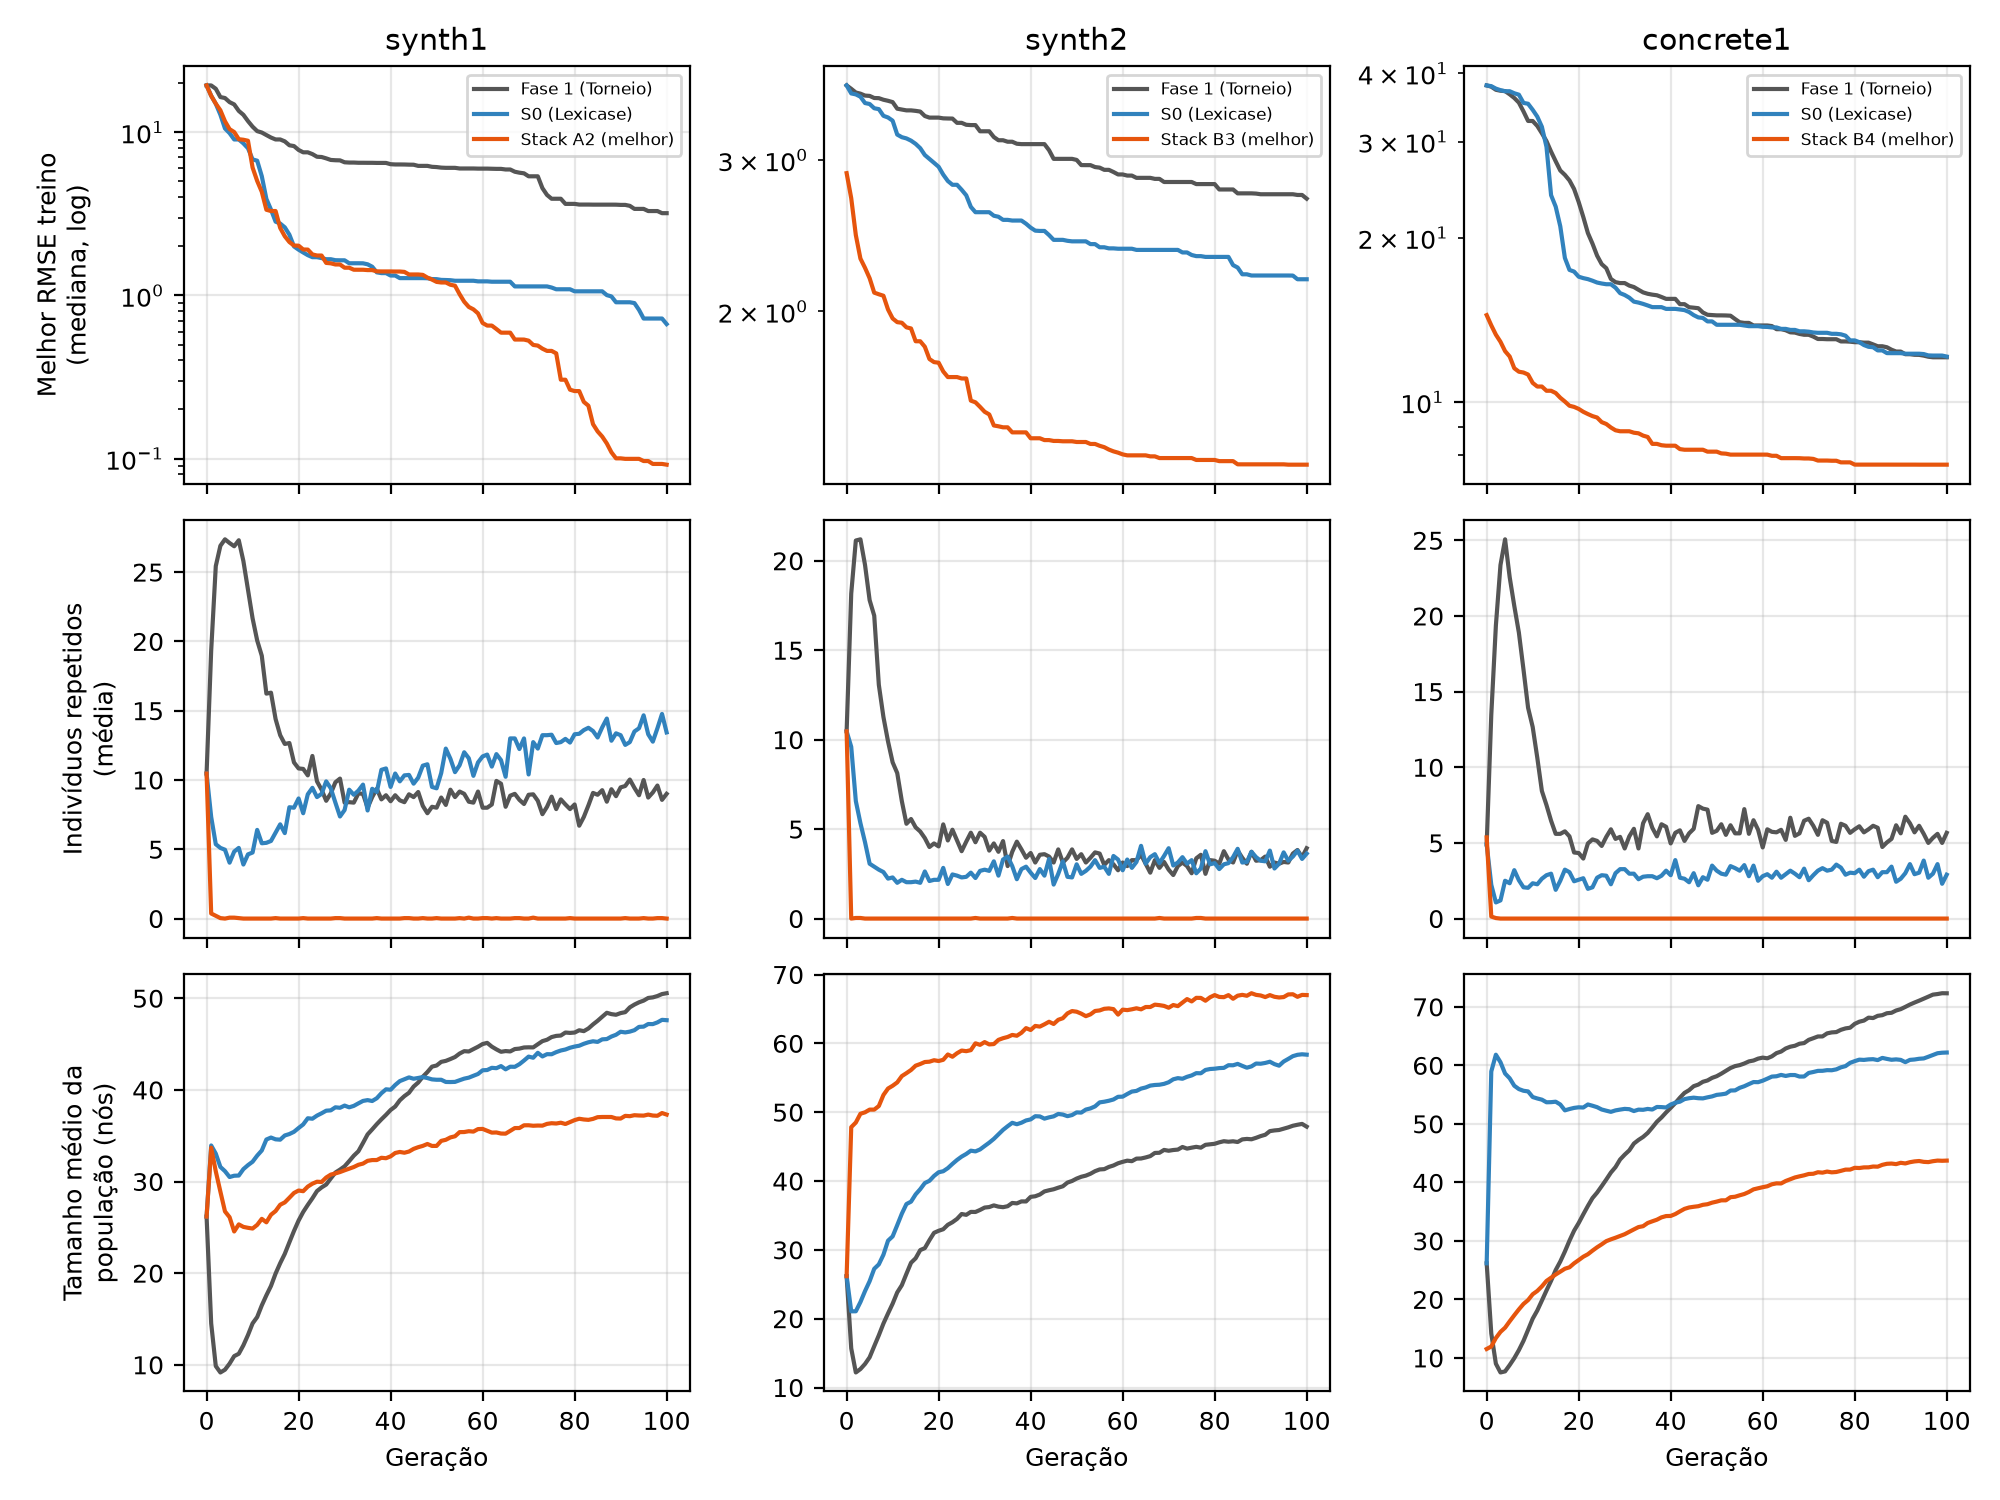
\includegraphics[width=0.7\linewidth]{f2_dinamica_comparada.png}
  \caption{Comparação da dinâmica evolutiva ao longo de 100 gerações entre a
           Fase~1 (torneio, cinza), Estado Atual (\cfg{S0} $\eps$-lexicase, azul)
           e Melhor Modelo da Fase~2 (laranja). Linhas representam a média
           populacional sobre 30 execuções.}
  \label{fig:f2_dinamica}
\end{figure}

\begin{enumerate}
  \item \textbf{População e Gerações:}
        A confirmação da hipótese H4 demonstrou por que uma população
        panmítica com pelo menos 100 indivíduos é crítica: ao fragmentar
        \code{pop=100} em 4 ilhas de 25, a $\eps$-lexicase perde o poder de
        manter especialistas em casos de teste variados. Quanto ao tempo de
        convergência, enquanto na Fase~1 a busca estagnava na geração~80, as
        intervenções da Fase~2 mantêm a evolução ativa até as gerações 88--96,
        ao mesmo tempo em que reduzem o tempo computacional médio: no
        \code{concrete1}, o tempo por execução caiu de $44.2$~s (\cfg{S0}) para
        $11.5$~s (\cfg{Stack~B4}) graças à forte redução no tamanho das árvores.
  \item \textbf{Dinâmica de Operadores (Cruzamento vs. Mutação):}
        Na Fase~1, constatou-se que o crossover operava como macromutação
        destrutiva em $89\%$ das vezes. A introdução de H2 ($\pc=0.7,\pmut=0.15$
        com mutação mista) validou diretamente a recomendação sugerida pelas
        varreduras da Fase~1. A mutação mista permitiu pequenos ajustes
        lineares e locais sem ruptura topológica, elevando a taxa de sucesso
        global das mutações para $43.5\%$ no \code{synth1} e $65.1\%$ no
        \code{synth2}.
  \item \textbf{Diversidade e Indivíduos Repetidos:}
        A segunda linha da \cref{fig:f2_dinamica} revela a drástica diferença:
        no torneio da Fase~1 ocorria um pico agudo de $\approx 25$ clones na
        geração~5; no \cfg{S0} a diversidade era melhor, mas acumulava até
        $13.4$ clones no final. Com a inclusão de \code{dedup} (H3), a contagem
        de indivíduos repetidos caiu a \textbf{zero absoluto} a partir da
        geração~2 em todas as bases, forçando 100\% do orçamento evolutivo a
        explorar árvores sintaticamente distintas.
  \item \textbf{Controle de Bloat e Tamanho das Árvores:}
        Na terceira linha da \cref{fig:f2_dinamica}, observa-se que no
        Baseline e no \cfg{S0} o tamanho médio cresce descontroladamente
        rumo ao teto de profundidade ($50.5$ a $72.3$ nós). Com a parcimônia
        lexicográfica (H5) e o \emph{Linear Scaling} (H6a), as árvores
        estabilizam em platôs muito inferiores: $35.9$ nós no \code{synth1}
        ($-23\%$ vs F1) e $43.3$ nós no \code{concrete1} ($-42\%$ vs F1),
        eliminando completamente os introns redundantes.
  \item \textbf{Estabilidade Treino vs. Teste e Generalização:}
        A razão mediana de generalização ($\text{RMSE}_{\text{teste}} / \text{RMSE}_{\text{treino}}$)
        caiu de $1.34$ (Fase~1) para $1.10$ no \code{synth1}, e no \code{concrete1}
        atingiu a paridade exata ($1.00$, $\text{gap} = 0.026$). No \code{synth2},
        onde ocorriam explosões de $415$, a razão mediana caiu de $2.56$
        (\cfg{S0}) para $1.07$ (\cfg{Stack~B3}), extinguindo o sobreajuste
        patológico.
\end{enumerate}
